\subsection{Crittosistema RSA}
Nel 1978 in \cite{RSA78} Rivest, Shamir e Adleman hanno proposto un crittosistema per la cifratura e la firma dei messaggi basato sulla crittografia asimmetrica.\\
Come vedremo nelle Figure successive il crittosistema si basa su tre funzioni principali: funzione di generazione delle chiavi, funzione di encryption e funzione di decryption.\\
Nella modellazione UML ogni oggetto rappresenta le funzioni matematiche utilizzate dalle tre funzioni.\\ 
L'oggetto Memory viene utilizzato dalla funzione di generazione delle chiavi per salvare le informazioni riguardo la chiave pubblica e la chiave privata necessarie alle funzioni di encryption e decryption.\\  

\begin{figure}[h!] 
    \centering 
    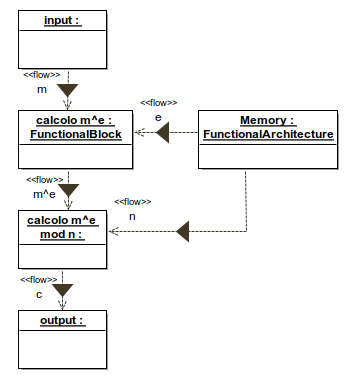
\includegraphics[scale=0.5]{../img/RSA/Encryption_Object_diagram.png} 
    \caption{Funzione di encryption} 
\end{figure}

\begin{figure}[h!] 
    \centering 
    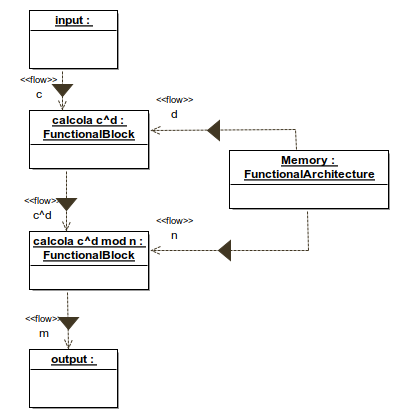
\includegraphics[scale=0.5]{../img/RSA/Decryption_Object_diagram.png} 
    \caption{Funzione di decryption} 
\end{figure}
\begin{figure}[h!] 
    \centering 
    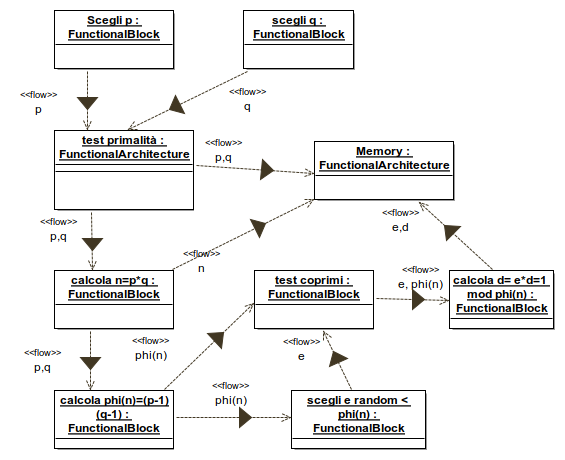
\includegraphics[scale=0.5]{../img/RSA/Key_Generation_Object_diagram.png} 
    \caption{Generazione delle chiavi} 
\end{figure}

\clearpage
\subsubsection*{Tool di verifica}
A seguito della modellazione UML del crittosistema RSA è possibile utilizzare il file .xmi estratto, visibile nel Listing \ref{lst:rsa1}\footnote{\label{note:c}Listing presentati in Appendice \ref{app:rsa}} per generare il file delle strutture Listing \ref{lst:rsa2}\textsuperscript{\ref{note:c}}.\\
In questo caso ci troviamo però in un caso particolare per il tool di conversione perch\'e il tool di analisi VerifPal utilizza un attaccante del modello Dolev-Yao, il quale non è in grado di rompere le primitive crittografiche, ed inoltre lo stesso VerifPal ci fornisce le primitive di encryption e decryption senza dover implementare nulla.\\
Per questo motivo deve essere l'utilizzatore a modellare il file da dare in input al tool di verifica a mano, andando ad ipotizzare uno scenario in cui viene utilizzato RSA:
\lstinputlisting[label={lst:nssk.vp},caption={File nssk.vp},language=vp, breaklines= true]{../code/verifpal/rsa.vp}
Come vediamo nel Listing \ref{lst:rsa3}\footnote{\label{note:d}Listing presentati in Appendice \ref{app:rsa}} il risultato della verifica sulla confidenzialità del messaggio \textbf{m\_b} viene preservata, questo perch\'e è il risultato della decryption con la chiave privata del principal e non è mai transitato in chiaro nella rete, ma viene trovato un problema di autenticazione per il messaggio \textbf{e\_2}, questo perch\'e per come è stato modellato il protocollo, l'attaccante può fingersi il secondo partecipante al protocollo andando a creare una coppia chiave pubblica-privata e inviare la sua chiave pubblica al posto di quella del reale partecipante.\\
La stessa situazione si verifica con la modellazione in Applied Pi Calculus (Listing \ref{lst:rsa4}\textsuperscript{\ref{note:d}}) come si può vedere dai risultati ottenuti con ProVerif (Listing \ref{lst:rsa5}\textsuperscript{\ref{note:d}}).\\
Ovviamente cambiando il tipo di scenario, ad esempio facendo in modo che le chiavi pubbliche siano certificate da una Public Key Infrastructure, i due tool di verifica automatica non rileveranno nessun tipo di problema riguardo autenticazione e confidenzialità.\\
Un metodo semplice di modellare questo nuovo scenario è quello di utilizzare una guardia sulle chiavi pubbliche scambiate dai principal, in modo che l'attaccante non possa n\'e leggerle, n\'e modificarle: 
\begin{lstlisting}[language=vp,mathescape]
    Alice -> Bob : [ga]
    Bob -> Alice : [gb]
\end{lstlisting}
\newpage